\documentclass[letterpaper,12pt]{article}
\usepackage{array}
\usepackage{threeparttable}
\usepackage{geometry}
\geometry{letterpaper,tmargin=1in,bmargin=1in,lmargin=1.25in,rmargin=1.25in}
\usepackage{fancyhdr,lastpage}
\pagestyle{fancy}
\lhead{}
\chead{}
\rhead{}
\lfoot{}
\cfoot{}
\rfoot{\footnotesize\textsl{Page \thepage\ of \pageref{LastPage}}}
\renewcommand\headrulewidth{0pt}
\renewcommand\footrulewidth{0pt}
\usepackage[format=hang,font=normalsize,labelfont=bf]{caption}
\usepackage{listings}
\lstset{frame=single,
  language=Python,
  showstringspaces=false,
  columns=flexible,
  basicstyle={\small\ttfamily},
  numbers=none,
  breaklines=true,
  breakatwhitespace=true
  tabsize=3
}
\usepackage{amsmath}
\usepackage{amssymb}
\usepackage{amsthm}
\usepackage{harvard}
\usepackage{setspace}
\usepackage{float,color}
\usepackage[pdftex]{graphicx}
\usepackage{hyperref}
\hypersetup{colorlinks,linkcolor=red,urlcolor=blue}
\theoremstyle{definition}
\newtheorem{theorem}{Theorem}
\newtheorem{acknowledgement}[theorem]{Acknowledgement}
\newtheorem{algorithm}[theorem]{Algorithm}
\newtheorem{axiom}[theorem]{Axiom}
\newtheorem{case}[theorem]{Case}
\newtheorem{claim}[theorem]{Claim}
\newtheorem{conclusion}[theorem]{Conclusion}
\newtheorem{condition}[theorem]{Condition}
\newtheorem{conjecture}[theorem]{Conjecture}
\newtheorem{corollary}[theorem]{Corollary}
\newtheorem{criterion}[theorem]{Criterion}
\newtheorem{definition}[theorem]{Definition}
\newtheorem{derivation}{Derivation} % Number derivations on their own
\newtheorem{example}[theorem]{Example}
\newtheorem{exercise}[theorem]{Exercise}
\newtheorem{lemma}[theorem]{Lemma}
\newtheorem{notation}[theorem]{Notation}
\newtheorem{problem}[theorem]{Problem}
\newtheorem{proposition}{Proposition} % Number propositions on their own
\newtheorem{remark}[theorem]{Remark}
\newtheorem{solution}[theorem]{Solution}
\newtheorem{summary}[theorem]{Summary}
%\numberwithin{equation}{section}
\bibliographystyle{aer}
\newcommand\ve{\varepsilon}
\newcommand\boldline{\arrayrulewidth{1pt}\hline}


\begin{document}

\begin{flushleft}
  \textbf{\large{Problem Set 2}} \\
  MACS 40200, Dr. Evans \\
  Nobuyuki Bambi Furuta
\end{flushleft}

\vspace{5mm}

\noindent\textbf{Problem 1}\\
\textbf{(a)} Mean: 720.278, Median: 172.210, Max: 227967.25, Min:0.01, Standard Deviation: 3972.664\\
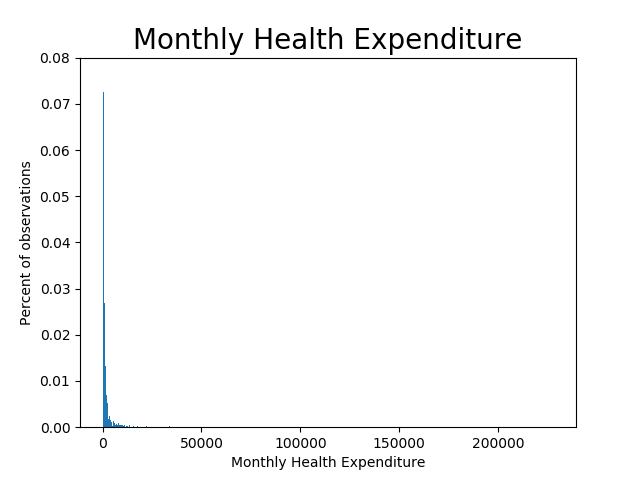
\includegraphics[width=5in]{ps2hist1}\\
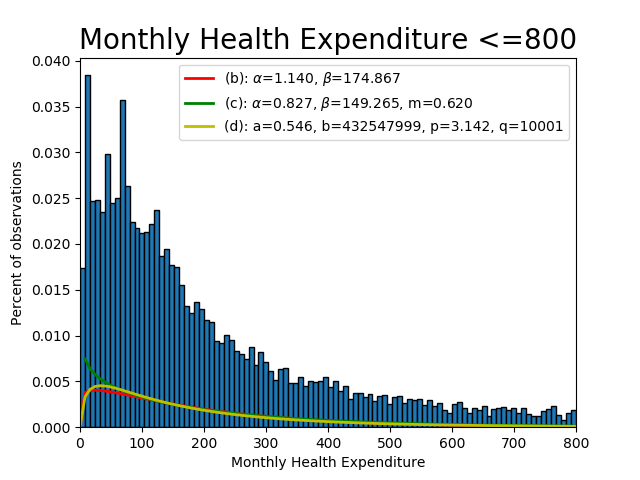
\includegraphics[width=5in]{ps2hist}\\
The second histogram is preferred because the mean is around 720 and most of the data are concentrated below mean. In addition, it takes away outliers such as 227967.\\ \\
\textbf{(b)} $\hat{\alpha}= 1.13976691235,  \hat{\beta}= 174.866836155, lnL= -56732.5986796$ \\ 
The estimated gamma distribution is depicted in the graph above with the red line. \\ \\
\textbf{(c)} $\hat{\alpha}= 0.826528658566,  \hat{\beta}= 149.264584308, \hat{m}= 0.618997875459, lnL= -56732.5986796$ \\
The estimated generalized gamma distribution is depicted in the graph above with the green line. \\ \\
\textbf{(d)} $\hat{a}= 0.545045409007,  \hat{b}= 432528268.017, \hat{p}= 3.16725263428, \hat{q}= 9999.89896562, lnL= -56800.0038081$ \\
The estimated generalized beta 2 distribution is depicted in the graph above with the yellow line. \\ \\
\textbf{(e)} p-value with the gamma distribution: 1.0 \\ p-value with the generalized gamma distribution: 1.0 \\ \\
\textbf{(f)} Using the generalized beta 2 distribution, the probability that one has a monthly health care claim for more than \$1,000 is 0.01182126643710546. \\ With the gamma distribution, it is 0.00457132368760782. \\ \\
Please see the attached Jupyter Notebook for the detail and codes used. I suppose that my calculation for the generalized gamma distribution is wrong, because it provided the weird estimated line. \\ \\
\end{document}